
\begin{frame}
\frametitle{Solutions - Virtualisation}
\begin{redbox}
\textbf{Virtualisation}
\begin{itemize}
    \item Divides physical computer resources into a series of virtual environments.
    \item Software directly shares a host machine's hardware.
    \item This is NOT the same as emulation!
\end{itemize}
\end{redbox}
\begin{yellowbox}
\textbf{Containerisation}
\begin{itemize}
    \item Virtualisation at OS-level.
    \item Software, along with its prerequisite OS libraries and dependencies, is packaged into a container.
    \item \textbf{Container:} A single executable that can run consistently on ANY system infrastructure.
\end{itemize}
\end{yellowbox}

\end{frame}

\begin{frame}
\frametitle{Containerisation - Advantages and Disadvantages}
\begin{theorembox}
\textbf{Advantages}
\begin{itemize}
    \item Improves scalability and utilisation of resources.
    \item Less overhead $\rightarrow$ highly portable.
    \item Host's kernel shared by all containers.
    \item Each container isolated during its runtime.
\end{itemize}
\end{theorembox}
\begin{redbox}
\textbf{Disadvantages}
\begin{itemize}
    \item Kernel vulnerability $\rightarrow$ security risk to all containers.
    \item Complex to manage large volumes of containers.
    \item Suboptimal performance for resource-intensive workloads.
\end{itemize}
\end{redbox}
\end{frame}

\begin{frame}
\frametitle{Containerisation vs VMs - Performance comparison}

\begin{figure}
  \centering

  \begin{subfigure}{0.48\textwidth}
    \centering
    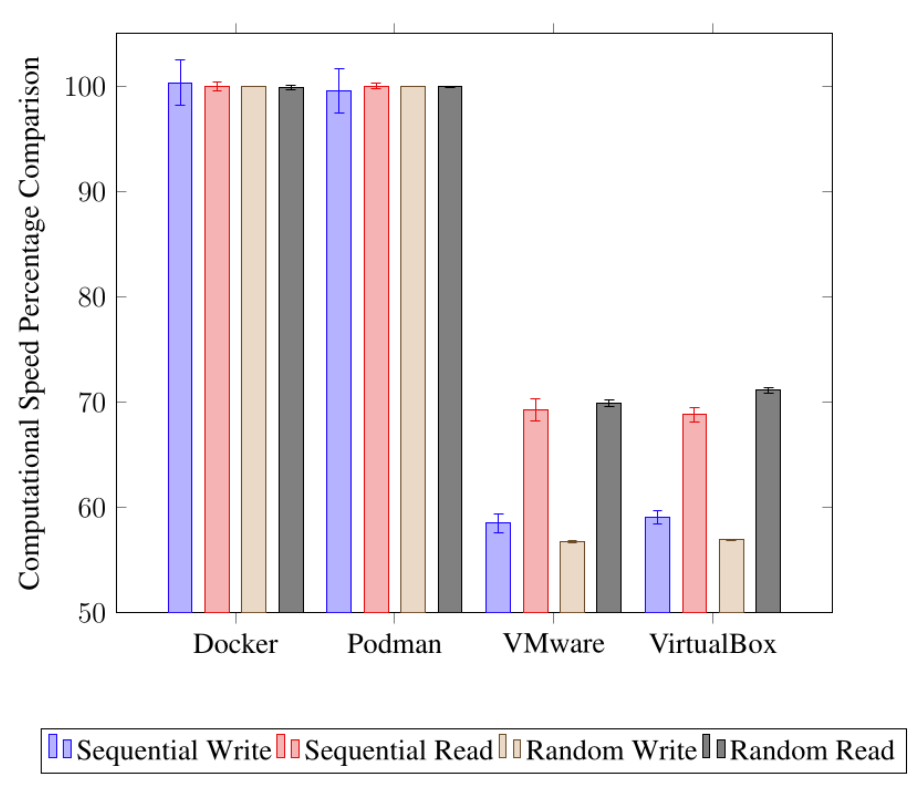
\includegraphics[width=2.2in]{section4/figs/mem_throughput.png}
    \caption{Memory throughput}
  \end{subfigure}\hfill
  \begin{subfigure}{0.48\textwidth}
    \centering
    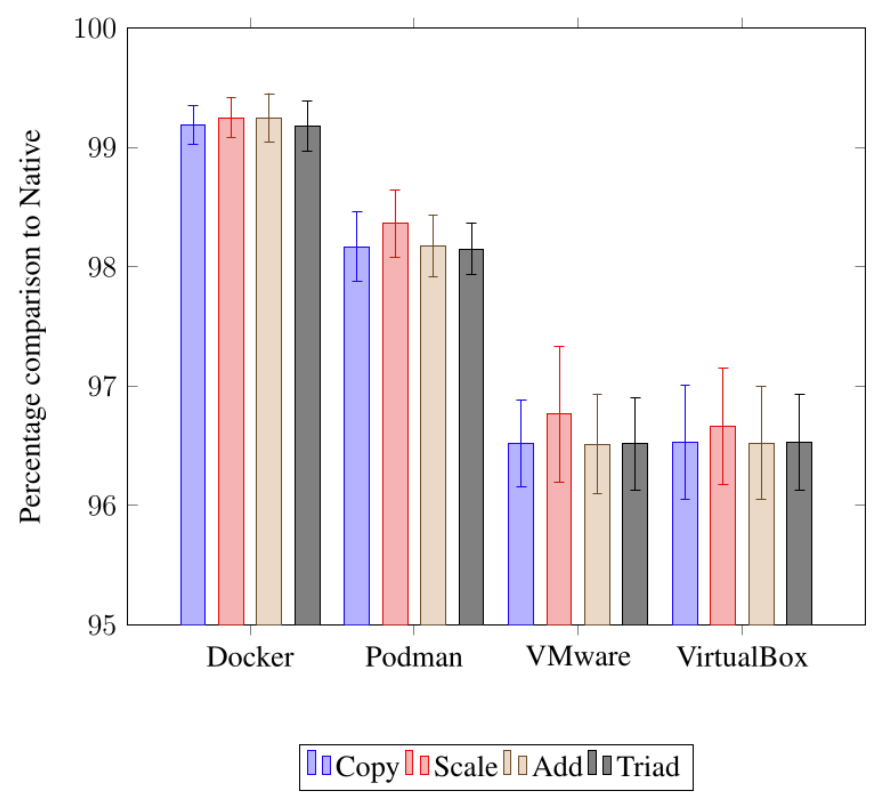
\includegraphics[width=2.05in]{section4/figs/STREAM_benchmark.png}
    \caption{Performance benchmark}
  \end{subfigure}

  \caption{Performance comparisons between containerisation (Docker, Podman) and VMs (VMware, VirtualBox)}
\end{figure}

\end{frame}

\begin{frame}
\frametitle{Containerisation - Evaluation}
\begin{theorembox}
\begin{itemize}
    \item \textbf{Stability} - Extremely stable
    \item \textbf{Performance} - Very limited overhead
    \item \textbf{Features} - 
    \item \textbf{Updates} - Dependent on host OS
\end{itemize}
\end{theorembox}
\end{frame}



